%%「論文」,「レター」,「レター(C分冊)」,「技術研究報告」などのテンプレート
%% v3.4 [2023/09/12]
%% 1. 「論文」
\documentclass[paper]{ieicej}
\usepackage{hyperref}  % クリック可能リンク用(任意)
\usepackage[hyphenbreaks]{breakurl}
\usepackage{url}       % URL表示用
\usepackage{cite}      % 数字で引用するため
\usepackage{enumitem}  % 数字の列挙を行うため 
\usepackage{tabularx}  % preamble に追加
\usepackage{booktabs}  % 表に罫線を入れる。
% \usepackage{rotating}  % page幅いっぱいに表を表示
% \usepackage[numbers]{natbib} % 数字で引用
%\documentclass[invited]{ieicej}% 招待論文
%\documentclass[survey]{ieicej}% サーベイ論文
%\documentclass[comment]{ieicej}% 解説論文
\usepackage[dvipdfmx]{graphicx,xcolor}
%\usepackage[dvips]{graphicx}
\usepackage[fleqn]{amsmath}
%\usepackage{amsthm}
\usepackage{newtxtext}% 英数字フォントの設定を変更しないでください
\usepackage[varg]{newtxmath}% % 英数字フォントの設定を変更しないでください
%\usepackage{amssymb}
%\usepackage{bm}

\setcounter{page}{1}

\field{A}
\jtitle{ダンス動画への音声・視覚情報付与による\\低学年児童・幼児向けダンス習得支援システム}
\etitle{A Dance Learning Support System for Lower-Grade and Preschool Children Using Audio and Visual Aids in Dance Videos}
\authorlist{%
 \authorentry{晴山 洋人}{Hiroto Hareyama}{A}\MembershipNumber{}
 \authorentry{長谷川 忍}{Shinobu Hasegawa}{B}\MembershipNumber{}
 %\authorentry{和文著者名}{英文著者名}{所属ラベル}\MembershipNumber{}
 %\authorentry[メールアドレス]{和文著者名}{英文著者名}{所属ラベル}\MembershipNumber{}
 %\authorentry{和文著者名}{英文著者名}{所属ラベル}[現在の所属ラベル]\MembershipNumber{}
}
\affiliate[A]{*}{*}
\affiliate[B]{北陸先端科学技術大学院大学 先端科学技術研究科}{Japan Advanced Institute of Science and Technology}
%\affiliate[所属ラベル]{和文所属}{英文所属}
%\paffiliate[]{}
%\paffiliate[現在の所属ラベル]{和文所属}
\jalcdoi{???????????}% ← このままにしておいてください

\begin{document}
\begin{abstract}
    本研究は, 見本動画を用いたダンス練習が一般化する一方, 児童・幼児が動画視聴のみで動作のタイミングや姿勢を正しく理解することが難しいという課題に着目した. 特にダンスの基本的な要素である, 姿勢を一瞬停止させる「止め」の動作に焦点を当て, 低学年児童・幼児を対象としたヒップホップダンス習得支援システムを開発し, その有効性を検証した. 本システムは, 音響・動画像解析により動画から「止め」のタイミングと姿勢を自動検出するコアエンジンと, 検出結果に基づきオノマトペ音声や視覚情報を付与するUIシステムから構成される. 評価実験では,コアエンジンの最適手法を同定し, UIシステムを用いて児童・幼児の練習効果を専門家が評価し, Wilcoxonの符号付順位和検定による統計的検討を行った. その結果, 短期練習では有意差は得られなかったものの, 女子のダンス経験者において「止め」の可視化が理解促進に寄与した可能性が示唆された. また, アンケートでは高い受容性が確認され, 特に視覚情報の有効性が顕著であった. 以上より, 本研究は従来研究で注目されなかった「止め」の自動検出技術を応用し, 児童・幼児向けダンス支援の新たな可能性を示すものである. 
%和文あらまし 500字以内
\end{abstract}
\begin{keyword}
    ダンス練習, 自動検出, 児童・幼児, 音声付与, 視覚情報付与
%和文キーワード 4〜5語
\end{keyword}
\begin{eabstract}
    This study proposes a hip-hop dance learning support system for young children, addressing difficulties in understanding timing and posture from videos alone. Focusing on the fundamental “stops” pose, the system combines automatic stops detection using audio-visual analysis with a UI providing onomatopoeic cues and visual feedback. Expert evaluations and Wilcoxon tests showed no overall short-term significance but suggested benefits for experienced girls, with strong user acceptance. These findings indicate the potential of stops detection for early childhood dance education.
%英文アブストラクト 100 words
\end{eabstract}
\begin{ekeyword}
    dance practice, automatic detection, children, audio support, visual support
%英文キーワード
\end{ekeyword}
\maketitle
\begin{figure*}[t]  % ← *付き
  \centering
  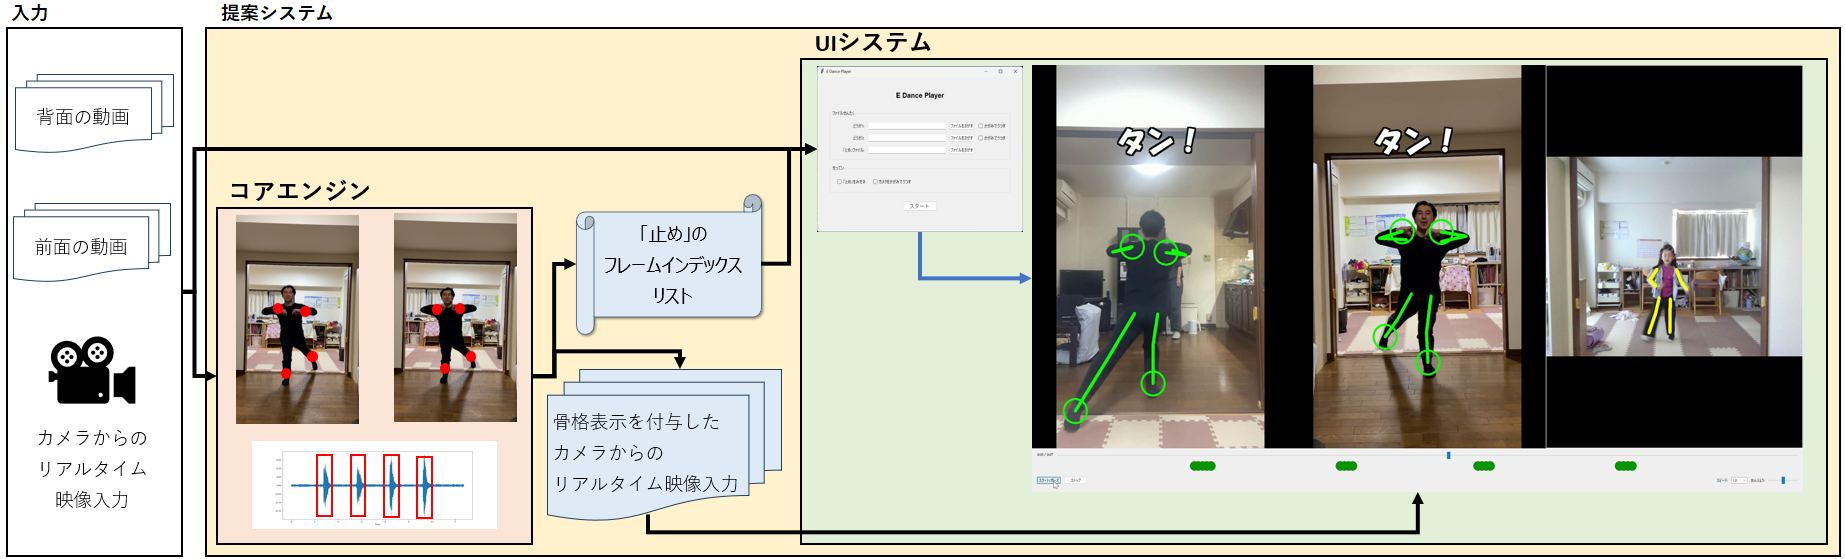
\includegraphics[width=\textwidth]{./images/summary.png}
  \caption{提案手法のシステム概要}
  \label{fig:summary}
  \begin{flushleft}
    \footnotesize 見本となる(ダンス指導者の)動画からコアエンジンを通して「止め」のフレームインデックスリストを抽出する. また, 同じ動画と同期して撮影したその背面の動画をUIシステムで指定して入力する. 最後に, 見本の前面・背面の動画と, カメラからのリアルタイム入力にコアエンジンの処理を合わせた動画をUIシステムで表示する.
  \end{flushleft}
\end{figure*}

\section{はじめに}
\subsection{研究の背景}
近年, ダンスは教育・スポーツ・メディアなど多様な分野で注目を集めている. 小学校ではリズムダンスが「表現運動」として取り入れられており \cite{ref1}, 2012年には中学校の保健体育でダンスが必修化された \cite{ref2}. また, 2024年のパリ五輪ではブレイキン(ブレイクダンス)が正式種目として採用されている \cite{ref3}. さらに, 2020年には日本初のプロダンスリーグ「D.LEAGUE」 \cite{ref4}が開幕し, ダンスがプロスポーツとしての道を歩み始めた. これらの動向は, ダンスが社会的に広く認知され, さまざまな世代に浸透していることを示している. このような社会的関心の高まりを背景に, 児童・幼児におけるヒップホップダンスの人口が増加している. 笹川スポーツ財団の調査 \cite{ref5} によれば, 4〜11歳(標本数:2,400人)を対象とした週1回以上のヒップホップダンス実施率は増加傾向にあり, 図 1 1に示すように2013年から2023年にかけて上昇し, 2.7\%から4.1\%に増加した. 住民基本台帳人口(4~11歳)(人)に上記実施率を乗じて算出した推計人口は24万人から33万人に増加している. \\
 ヒップホップダンスの基本的なリズムの取り方は, 膝を屈伸させて沈み込む「ダウン」と膝を伸ばして体を引き上げる「アップ」である\cite{ref7}. また, 基本的な動きの一つである「上肢のウェーブ動作」はウェーブを伝搬させる速度が一定, 振幅が一定で正弦波のように滑らかである. つまり, リズムをとりながら周期的に身体を「止め」る動作を循環的に行うのがヒップホップダンスの特徴である. \\
 児童・幼児はヒップホップダンス(以下, ダンス)を基本的な動きから段階的に習得していく. 基本的な動きは, 姿勢を一瞬静止させる「止め」の連続で構成されており, 各ステップのカウントにおける「止め」の動きを通じて振付を学んでいく. この「止め」の動きは, 上級者においてもキレやタメといった高度な表現を生み出す重要な技法である. \cite{ref6} \cite{ref7} たとえば, 次の動きへの移行前にポーズをとることで安定感や表現を強調する「Pose」や, 音楽のビートに合わせて身体を一瞬固定させる「Hit」といった手法がある. \\
 こうした動きを児童・幼児がダンスを習得する際には, ダンス教室などで指導者の動きを模倣することが一般的である. 内山はダンス学習の際に最もオーソドックスな方法は「模倣」であると述べている \cite{ref8}. また飯野らは上級者の指導の下, 鏡で自分の姿を見ながら修正するか, DVDなどの映像を見て真似るかのいずれかが主な練習方法であると主張している \cite{ref9}. ダンス教室では, 指導者は児童・幼児の前に立ち, 鏡越しに後ろ向きで踊る. その結果, 児童・幼児は指導者の背面の動きと鏡に映った左右反転した動きを同時に観察しながら, 身体を動かし, 振付を学んでいくことが行われている. またスマートフォンが普及した現代では, 指導者の動きを撮影し, その動画を家庭で確認しながら自主練習することも推奨されている. ダンスの技術を向上させるためには, 日々の練習が極めて重要である. 中でも, 動画を活用した自主練習は技術向上だけでなく, ダンスを楽しむうえでも欠かせない活動であると考えられる.  \\
 しかし, 動画を視聴するだけでは, 児童・幼児にとって「止め」のタイミングやその姿勢を正しく理解することは難しいと考えられる. 実際のダンス指導の現場では, 「タン・タン」などのオノマトペ(擬音語)を用いて動きのタイミングを伝え「止め」の姿勢について指導者が説明を交えて指導し, それを児童・幼児が実践することで, 段階的に振付を習得しているのが現状である. 
\subsection{研究の目的}
そこで本研究では, ヒップホップダンスを対象とし, ヒップホップダンスにおける「止め」の動きに着目する. 動画上の「止め」の瞬間に音声・視覚情報を付与することで, 児童・幼児のダンス習得を支援することを目的とする. まず, 児童・幼児が見本動画から「止め」の動きを自動で検出できるシステムを開発する. 次に, 「止め」の動きに対して, 音声, 記号, 文字といった情報を付与することで, 児童・幼児にとってより分かりやすく振付を理解できるようにするシステムを構築する. \\
 さらに, 上記のシステムを用いて, 音声・視覚情報を付与した動画と, 付与していない動画を用いた場合で, 児童・幼児のダンス習得に差が生じるかを検証する比較実験を行う. 
\subsection{本論文の構成}
本論文の構成は以下の通りである. まず第2章では本研究に関連する先行研究について述べる. 先行研究は大きく教育的観点, 支援システム関連, 骨格検出関連に大別される. 第3章では本研究の提案手法について述べる. また, 本研究の要件について述べ, 課題を明確化する. 第4章では提案手法の実装について述べる. 主に「止め」の動きを検出するシステムであるコアエンジンと児童・幼児に「止め」の動きの理解を促すUIシステムについて述べる. 第5章では提案システムを使用した実験及び評価について述べる. 第6章では最終的な成果と今後の課題について述べる. 
\section{関連研究}
本章では, ダンス習得に関する先行研究について, 教育的観点からの研究とシステムを活用した研究, 及び「止め」の検出の際に使用する骨格検出に関する研究に大別して概説する.
\subsection{教育的観点からのダンス習得に関する研究}
教育的観点からのダンス習得に関する研究では, 幼児や児童を対象とした効果的な指導法や学習過程に関する実践的な知見が報告されている. たとえば, 指導段階を明確に区分して考察する研究 \cite{ref10}や, 指導者と児童が「よい動き」について共通理解を持つことで技能向上を図る研究 \cite{ref11}, 特定のダンス技法の習得方法に焦点を当てた研究 \cite{ref12}などがある.\\
 亀山は幼稚園年長児(5~6歳)を対象にリズムダンスの習得過程を「①導入期, ②練習期, ③葛藤期, ④変化期, ⑤発表期」の5段階に分類している \cite{ref10}. 特に③葛藤期において, 子どもが音やリズムを感じながら, 自身の身体を通して動きを獲得していく過程が重要であることが示されている.\\
 湯浅らは, 小学校低学年におけるリズム遊びの指導において, 「よい動き」に対する合意形成を行うことで, 児童の動作パフォーマンスの向上が認められたと報告している \cite{ref11}. さらに湯浅は, 小学校2年生(7~8歳)に対するリズム系ダンス授業の実践を通じて, 児童同士が「よい動き」を共通理解することで, 着目する身体部位が明確化され, さらに他者と関わりながら踊ることで, ダンス技能の習得が促進されると主張している \cite{ref12}.\\
 本研究に関連の深い研究として, 高田は, 幼児期および児童期初期の発達段階に応じたダンス実践を報告しており, 幼児におけるダンス習得には「動作の分割(上半身と下半身を別々に動かすこと)」や「音楽に合わせて踊る時間の確保」が重要であるとしている \cite{ref13}. ただし, 各ステップにおける「止め」の動きに関する分割については具体的に言及されていない.\\
 天野らは, 「言語のみ」「オノマトペのみ」「言語とオノマトペの併用」「カウントのみ」の4種類の指導方法が動作習得過程に与える影響について, 比較実験を通じて検討した. これらの指導方法はいずれも, 動画に音声を付加する形で提示された. その結果, 初めから「言語とオノマトペ」を併用して指導する場合, 学習者が情報過多になる可能性が示唆された. また, 初見の振り付けを学習する際には, まず全体の流れを把握し, その後に詳細な動作を段階的に習得するという学習プロセスが有効であることが示唆された \cite{ref14}. また, \cite{ref14}の中で斎藤ら \cite{ref15}の研究との違いが論じられている. 斎藤ら \cite{ref15}の研究は動画に「音声のみ」, 「文字のみ」で動画にオノマトペを付与するもので, \cite{ref14}ではその「音声のみ」のオノマトペ付与をより深く研究したものと言える. \cite{ref14}の研究の中で, 「音声のみ」のオノマトペ付与効果が限定的であったことから, 斎藤ら \cite{ref15}の「文字のみ」オノマトペ付与でダンス習得効果が向上したことと比較し, 動画による学習においては, 聴覚情報よりも視覚情報の方が学習に強く影響を及ぼす可能性を主張している. これは, 言語やオノマトペを文字として画面表示することがダンス習得に影響を及ぼすことを示唆している. \\
 最後に, 本研究と関連の深い先行研究との共通点及び相違点を以下に示す. \\
\textit{<共通点>}
\begin{itemize}[nosep]
  \item 児童・幼児のダンス習得において動作の分割が重要であることが報告されている. 
  \item ダンス習得において, オノマトペを音声として付与する影響を報告している. 
\end{itemize}
\textit{<相違点>}
\begin{itemize}[nosep]
  \item 動画の分割について述べられているが, 「止め」の動作に注目した分割については言及されていない.  
  \item \cite{ref14}ではオノマトペの音声付与のみの影響について言及しており, \cite{ref15}ではオノマトペの視覚提示の可能性が述べられている. しかし, 音声と文字表示の両方を付与した場合についての言及はない. 
\end{itemize}
\subsection{システムによるダンス習得に関する研究}
システムを活用したダンス習得支援に関する研究では, さまざまな提案がなされている. これらには, ダンス動画への視覚情報の付加による学習効果の検証 \cite{ref15}や, 動画の自動分割技術の応用 \cite{ref16}などが含まれる. \\
 田中らは, ストリートダンスの動作データを解析し, 動きの特徴を抽出した上で上級者との比較を行い, その結果を直感的に把握できる形で可視化するシステムを提案している \cite{ref17}. \\
 山内らは, Kinectとワイヤレスマウスを組み合わせたダンス学習支援システムを提案し, マウスによるタッピング操作を用いてリズム感の習得度合を定量的に判定可能とした \cite{ref18}.\\
 西脇らは, 学習意欲が高くないユーザーでもダンスの基礎やステップを習得できるよう, 習熟度に応じて動作判定やフィードバックを変化させるシステムを開発した \cite{ref19}. また, ユーザーが踊りながら間違いを修正できるよう, リアルタイムで音声によるフィードバックを行った. \\
 何らは, 適応型ダンス練習支援システム「FreeDance」を提案し, 三面壁型透明スクリーンを用いることで高い没入感を実現し, 学習者の動機づけを促進している \cite{ref20}. \\
 戸山らは, 撮影したダンス動画を加速度データに基づいて動作の単位に自動で分割し, その単位ごとに繰り返し再生可能なインタラクティブチュートリアルを実現している \cite{ref21}. 実験の結果, 初心者にとっては未加工の動画よりも本システムによる学習の方が振り付けを覚えやすいことが示された. \\
 本研究と関連の深い先行研究として, 斎藤らは, 漫画風オノマトペをダンス動画に視覚的に付与することで, ダンス習得効果が向上することを示した \cite{ref15}. 本研究においても同様の視覚的オノマトペの付加を行っているが, 音声と文字の両方を付与した際の比較については言及がない. \\
 また, Endoらは, ダンス動画から振り付けの短時間の動きを自動で分割する手法を提案しており, キーポイント間の速度変化を視覚特徴量として利用している \cite{ref16}. 本研究のように「止め」の動きの検出については言及されていない点, および幼児・児童向けのUI設計には対応していない点で差異がある. \\
 さらに, Andersonらは, 自己学習を支援するARミラー型インターフェース「YouMove」を提案している \cite{ref22}. 「YouMove」はユーザーの姿勢をリアルタイムに解析して見本との違いを可視化し, 動作の一時停止や繰り返し再生などの機能を備えている. 本研究でも同様に骨格推定や動画の一時停止・繰り返し再生機能を実装しているが, 見本動作の表示方法としては, 重ね合わせ表示ではなく並行表示を採用している点で異なっている.\\
 最後に, 本研究と関連の深い先行研究との共通点及び相違点を以下に示す.\\
\textit{<共通点>}
\begin{itemize}[nosep]
  \item 動画にオノマトペを付与した場合の効果を示している. 
  \item ダンスの振り付けを自動で分割する手法について述べている. 
  \item 自己学習を支援するインターフェースを提案している. 
\end{itemize}
\textit{<相違点>}
\begin{itemize}[nosep]
  \item 動画にオノマトペの音声と文字両方を付与した場合の効果については述べられていない. 
  \item 「止め」の分割についての言及はない. 
  \item 見本動作の表示方法として, 重ね合わせではなく, 並行表示を採用している. 
\end{itemize}
\subsection{骨格検出に関する研究}
骨格検出(Pose Estimation)は, 画像または映像内の人体の関節位置を特定する技術である. 人体の動きや姿勢を機械が理解するための基盤技術として, 多くの研究が行われてきた. 初期には特徴点を用いた機械学習による分類が行われたが, 特にディープラーニングの進展により, リアルタイムで高精度な骨格検出が可能となり, さまざまな実用化が進んでいる. \\
 CaoらによるOpenPose \cite{ref23}は, 初めてマルチパーソン骨格検出をリアルタイムで実現したオープンソースのシステムである. Part Affinity Fields(PAFs)と呼ばれる空間的なベクトル場を導入することで, 複数人物に対する2次元姿勢推定を高精度でリアルタイムに行うことができる. ただし, リアルタイム処理についてはGPUを使用した場合に限り実現可能であることが報告されており, CPUのみでのリアルタイム実行は困難である.\\
 BazarevskyらによるMediaPipe \cite{ref24}は, Googleが開発したオープンソースのマルチモーダル機械学習フレームワークである. リアルタイムな画像処理および機械学習パイプラインの構築を支援するプラットフォームで, 手や顔の検出, 姿勢推定などの高精度な機能を備えている. 組み込み機器やスマートフォンでのリアルタイム推論を目的とした軽量なライブラリであり, CPUでもリアルタイムに実行可能である. 少ない計算リソースでも一定の精度で実行できることが確認できたため, 本研究ではMediaPipeを利用することとする.\\
 Xu らによるViTPose \cite{ref25}は, 人体姿勢推定のための新しいアーキテクチャであり, Vision Transformer(ViT \cite{ref26})を活用した手法である. このモデルは, 従来の畳み込みニューラルネットワーク(CNN)ベースのアプローチに比べ, 視覚的特徴の処理において高い効率性と精度を発揮する. ViTPoseは, 画像内の各関節位置を予測するために, トランスフォーマーの自己注意メカニズムを活用し, 物体の局所的およびグローバルな特徴を効果的に学習する. しかしながら, 環境構築が複雑で, 要求リソースも大きいことから本実装では採用しなかった. 
\section{提案手法}
\subsection{アーキテクチャ}
本研究は, 児童・幼児のダンス習得支援を目的として, 各ステップにおける「止め」の動作に着目し, 視覚および音声情報を付加することにより, 「止め」の姿勢およびタイミングの理解を促進するシステムの提案を行うものである. 特に, 「止め」の動作を視覚的に明確化し, 音声的な手がかりと組み合わせることで, 児童・幼児のダンス学習を効果的に支援することを目指す. \\
 図1に提案システムのアーキテクチャ図を示す. 入力として見本となる(ダンス指導者の)動画から「止め」のフレームインデックスリストを抽出する. また, 同じ動画と同期して撮影したその背面の動画をUIシステムで指定して入力する. 入力動画の「止め」のフレームに音声・視覚情報を付与し, カメラからのリアルタイム入力を合わせてUIシステムで表示する. カメラからの表示には「止め」の抽出と同じアルゴリズムを用いて視覚情報を付与する. \\
 提案システムは, 以下の2つの主要な機能で構成される.
\begin{itemize}[nosep]
  \item コアエンジン:見本となる(ダンス指導者の)ダンス動画を入力とし, 音響情報および動画像情報を解析することで, 「止め」の動作を自動的に検出する. 
  \item ユーザーインターフェースシステム(UIシステム):検出された「止め」のフレームに対して, 視覚および音声情報を付与することで, 児童・幼児が動作の内容とタイミングを理解しやすくなるよう支援する. 
\end{itemize}
 コアエンジンでは, 入力されたダンス動画から音響情報および動画像情報を抽出する. 音響情報に関しては, 周期的な音のピークを検出し, 「止め」のタイミングの候補フレームを抽出する. 一方, 動画像情報においては, 骨格推定によりダンス上級者の手首および足首のキーポイントを検出し, 各フレーム間における移動速度がゼロとなる箇所を「止め」の姿勢候補として抽出する. これら双方の候補が一致する動画フレームを「止め」の動作として確定する.  \\
 UIシステムでは, 検出された「止め」の動画フレームに対して, オノマトペによる音声情報および記号・文字による視覚情報を重ね合わせる. また, カメラからのリアルタイム入力にコアエンジンと同じアルゴリズムを用いて骨格情報を視覚的に付与する. これにより, 児童・幼児は視覚と聴覚の両面から「止め」のタイミングと姿勢を直感的に理解することが可能となる. \\
\subsection{要件}
本研究で解決すべき課題は以下の通りである.\\
\subsubsection{コアエンジンの課題}
\begin{itemize}[nosep]
  \item 音響情報により「止め」のタイミングを検出する. 
  \item 動画像情報により「止め」のタイミングの姿勢を検出する. 
\end{itemize}
\subsubsection{UIシステムの課題}
\begin{itemize}
  \item 検出した「止め」の動作に音声・視覚情報を付与する.  
\end{itemize}
\section{実装}
\subsection{コアエンジン}
コアエンジンの入力と出力は以下である. 
\begin{itemize}[nosep]
  \item 入力:動画(.mp4)ファイル
  \item 出力:「止め」の動作を行っている動画フレームインデックスのリスト
\end{itemize}
 コアエンジンでは, 音響情報で検出したフレームと動画像情報で検出したフレームの共通フレームを「止め」の動作を行っている動画フレームとして検出し, その動画フレームのインデックスのリストを出力する. また, ダンス経験者とのディスカッションの中で, 「止ま」り始める部分についても「止め」の動作とするとよいとのアドバイスを受け, 共通フレームが連続3フレーム以下の場合は, 1フレーム前のフレームも「止め」のフレームとした. \\
 本研究での入力動画ファイルの条件は以下の通りとする. 
\begin{itemize}[nosep]
  \item 入力動画ファイルはBPM(Beats Per Minute)=90のダンス振り付けを撮影した動画である. 
  \item 入力動画ファイルのfpsは30.0である. 
  \item 入力動画ファイルはメトロノーム音が鳴っている中で撮影した動画である. 
  \item メトロノーム音が鳴っているタイミングが「止め」のタイミングの候補となる. 
  \item メトロノーム音が動画内の音響情報において主要な要素を占めており, 他には足音などの微小な環境音がわずかに含まれるのみである. 
\end{itemize}
\subsubsection{音響情報による「止め」のタイミングの検出}
音響情報による「止め」のタイミング検出手法として以下の2手法を実装する. \\
\textit{<振幅特徴ベース>}\\
 入力動画の周期的な音響情報(メトロノーム音)にて音の振幅がピーク(局所最大値)となる動画のフレーム番号を検出する. 音の振幅は動画内のフレーム数を$N$, 動画1フレーム単位での音の振幅$x_i(i=1,\dots,N)$とした時, 以下2つの条件を満たすフレームをピークとして検出する. \\
 閾値(振幅の高さ$h$の条件):$h=\mu+\sigma$ \\
 ここで$\mu$と$\sigma$は以下の式で表される.
\begin{equation}
  \mu=\frac{1}{N}\sum_{i=1}^{N} x_{i}
\end{equation}
\begin{equation}
  \sigma=\sqrt{\frac{1}{N} \sum_{i=1}^{N}(x_{i}-\mu)^2}
\end{equation}
 閾値で検出したフレームの前後1フレームもピークとする. \\
\textit{<自己相関関数ベース>}\\
 自己相関関数を用いた手法はまず対象とする音声ファイルから単一チャネル(モノラル)として信号$y[n]$を抽出する. サンプリング周波数を$f_s$とする. 信号の周期的構造を明らかにするために, 自己相関関数$R[k]$を用いる. これは以下の式で定義される.
\begin{equation}
  R[k]=\sum_{n=0}^{N-1-k} y[n] \cdot y[n+k] \quad (0 \leq k \leq N)
\end{equation}
ここで$N$は信号の長さである. 次に自己相関関数$R[k]$からpeak位置を検出する. このとき, メトロノームが打つ間隔(BPM=90より0.5秒程度)に基づき, peak間の最小処理を制限することで可検出を防ぐ.
\begin{equation}
  P_{\mathrm{auto}}=FindPeaks(R[k],distance= f_{s}\cdot0.5)
\end{equation} 
周期推定値は, 検出されたピーク間の中央値を用いて次のように求める. 
\begin{equation}
  T_{\mathrm{est}}=median(\Delta P_{\mathrm{auto}})
\end{equation} 
元の音響信号$y[n]$上で音のpeak位置を求める. peak検出においては, 次の2つの条件を課す:
\begin{itemize}[nosep]
  \item 信号の振幅が最大値の50\%以上であること(=メトロノーム以外の微小ノイズを除外)
  \item 推定周期の80\%以上の間隔でpeakを制限(=1打で複数のpeakを検出しない)
\end{itemize}
\begin{equation}
  \begin{split}
  P_{\mathrm{auto}}=FindPeaks(&y[n],\\
                     &height \geq 0.5 \cdot max(y),\\
                     &distance \geq 0.8 \cdot T_{\mathrm{est}})
  \end{split}
\end{equation} 
ここで, $P_{\mathrm{auto}}$は音声サンプルインデックスのリストである. \\
動画のフレームレートを$f_{\mathrm{fps}} [\mathrm{fps}]$としたとき, サンプル番号$n$は以下の式により対応するフレーム番号$f$に変換される. 
\begin{equation}
  f=\lfloor\frac{n}{f_{s}} \cdot f_{\mathrm{fps}} \rfloor
\end{equation}
以上により, 自己相関関数を用いてメトロノームが鳴るフレーム番号のリストを得る. peak検出にはScipy \cite{ref27}のfind\_peaks 関数を用いる.
\subsubsection{動画像情報による「止め」のタイミングの姿勢検出}
動画像情報による「止め」のタイミング検出手法として以下の3手法を実装する. これに先立ち, 前処理として各キーポイントの速度情報を算出する。まず, 骨格検出モデルMediaPipe \cite{ref24}を用いて左右手首・足首のキーポイントを検出する. 次に, 検出したキーポイントの動画フレーム間速度を算出する. フレーム$t$で検出した$i$番目のキーポイントの位置$(x_{i},y_{i})$を$k_{i}(t)\in\mathbb{R}^2$, 速度$v(t)\in\mathbb{R}^{(4 \times 2)}$の$i$番目の要素$v_{i}(t)\in\mathbb{R}^2$を以下の式で求める. 
\begin{equation}
  v_{i} (t)=|k_{i}(t)-k_{i}(t-1)|
\end{equation}
\textit{<閾値アルゴリズム>}\\
 上式で算出した速度$v(t)$が閾値以下のフレームを「止め」のタイミングの姿勢とした. 本研究では後述する予備実験により, 閾値の値を10[pixel/frame]とする. 
\textit{<Peak検出アルゴリズム>}\\
 peak検出では, まず各キーポイントの速度系列データ$(v_{i}(1),v_{i}(2),\dots,v_{i}(n))$に対して, 最小値$v_{i min}$及び最大値$v_{i max}$を用いたmin-max正規化を行う. 
\begin{equation}
  \hat{v}_{i}(t) =
  \begin{cases}
    \dfrac{v_{i}(t) - v_{i\ \mathrm{min}}}
          {v_{i\ \mathrm{max}} - v_{i\ \mathrm{min}}}
      & \text{if } v_{i\ \mathrm{max}} > v_{i\ \mathrm{min}}, \\
      & \quad t = 1,2,\dots,n \\[6pt]
    0 & \text{otherwise}
  \end{cases}
\end{equation}
また, $\hat{v}_{i}(t)$の$t$に対して平均をとることで統合信号$s_{t}=(s_{1},s_{2},\dots,s_{n} )$を構成する:
\begin{equation}
  s_{t}=\frac{1}{d}\sum_{j=1}^{d}\hat{v}_{i}(t),\text{for}\;t = 1,2,\dots,n
\end{equation}
ここで$d$は左右手首・足首のキーポイント位置$(x,y)$であるため, $d=8$となる. 統合信号を再びmin-max正規化した後, peak検出アルゴリズムを適用する. 本実装ではpeak検出アルゴリズムとしてScipy \cite{ref27} のfind\_peaks 関数を用いた. パラメータはpeak間の最小距離を15フレーム(fps30で約0.5秒), peakの顕著性(突出度)をノイズ除去のため0.3とした. 
\begin{equation}
  \mathcal{P} = \mathrm{FindPeaks}(
  \begin{aligned}[t]
    & s_{t}, \\
    & distance=15, \\
    & prominence=0.3)
  \end{aligned}
\end{equation}
得られたpeak位置の集合を$\mathcal{P}=(p_{1},p_{2},\dots,p_{k})$とすると, 各peak $p\in \mathcal{P}$の周辺$[p-w,p+w]$を動いている区間とみなし, ブール配列$h_{t}=(h_{1},h_{2},\dots,h_{n})$を次のように定義する.
\begin{equation}
  h_{t}=
  \begin{cases}
    1 & \text{if}\; \exists p \in \mathcal{P}, |t-p| \leq w\\
    0 & \text{otherwise}
  \end{cases}
\end{equation}
ここで$w=\lfloor \frac{distance}{2} \rfloor=7$である. 最終的に$h_{i}=0$すなわち動いている区間に属さないインデックス$t$を「止め」の区間とみなし, それらのインデックス集合を$\mathcal{L}$として抽出する. 
\begin{equation}
  \mathcal{L} = \{ t \in \{1,2,\dots,n\} \mid h_t = 0 \}
\end{equation}
\textit{<k-meansアルゴリズム>}\\
k-meansのクラスタリングでは, まず各キーポイントの速度系列データ(速度$v_{i}(1),v_{i}(2)\dots,v_{i}(n)$)に対して,以下のように標準化を行い, 平均0, 分散1の正規化済みデータを得る:
\begin{equation}
  \tilde{v}_{i}(t)=\frac{v_{i}(t)-\mu_{i}}{\sigma_{i}}(1 \leq t \leq n,1 \leq i \leq d)
\end{equation}
ここで$d=8$である. また, $\mu_{i}$及び$\sigma_{i}$は各キーポイントの要素(左右手首・足首の$(x,y)$)の平均と分散である. 標準化された$\tilde{v}(t)$に対して, クラスタ数$k=2$のk-meansクラスタリングを実行し, 各サンプル$t$が属するクラスタラベル$c_{i} \in \{0,1\}$を得る. 
\begin{equation}
  c_{i}=\text{argmin}_{k \in \{0,1\}} ‖\tilde{v}(t)-\mu_{k} ‖^2
\end{equation}
ただし, $\mu_{k}$はクラスタ$k$の中心である. クラスタ中心の各次元の平均値を計算し, 平均が大きいクラスタを「動作クラスタ」, 小さい方を「「止め」クラスタ」とする. クラスタ$k$の平均値は以下で定義される.:
\begin{equation}
  m_{k}=\frac{1}{d}\sum_{i=1}^d \mu_{k,j}
\end{equation}
ここで, $\mu_{k,j}$はクラスタ$k$の$i$番目の次元の中心値である. 平均$m_{0}$と平均$m_{1}$を比較し, $m_{1}>m_{0}$の場合はクラスタ1を「動作クラスタ」, そうでなければクラスタ0を「動作クラスタ」とする. クラスタラベルが「動作クラスタ」ではないサンプル$t$を抽出し, 昇順でソートしたものが「止め」のフレームインデックスリストである.
\subsection{UIシステム}
UIシステムの入力と出力は以下である. また, 図 4 1, 図2の通り実装した. 
\begin{itemize}[nosep]
  \item 入力:
  \begin{itemize}[nosep]
    \item 同期させて撮影した見本のダンス動画ファイル(.mp4)
    \begin{itemize}[nosep]
      \item 前面から撮影された動画ファイル(図 4 1(a))
      \item 背面から撮影された動画ファイル(図 4 1 (a))
    \end{itemize}
    \item コアエンジンで検出した「止め」の動作を行っている動画フレームインデックスのリスト(図 4 1 (c))
    \item カメラからの動画像(リアルタイム表示)(図2(c))
  \end{itemize}
  \item 出力:
  \begin{itemize}[nosep]
    \item 入力された動画ファイルに音声・視覚情報を付与した動画(図2 (a), (b))
    \item カメラからの動画像に視覚情報を付与したリアルタイム表示(図2 (j))
  \end{itemize}
\end{itemize}
 上記の”音声情報の付与”とは以下を行うことである.
\begin{itemize}[nosep]
  \item 「止め」のタイミングでオノマトペの音声情報を付与する. 
\end{itemize}
 上記の”視覚情報の付与”とは以下を行うことである. 
\begin{itemize}[nosep]
  \item 	左右の肩から手首, 腰から足首までに骨格表示を行う. 骨格表示は「止め」の姿勢では緑色になり, それ以外は黄色になる. (図2 (h))
  \item 「止め」の姿勢の際に左右手首・足首に丸の図形付与(図2(h))
  \item 「止め」の姿勢の際に漫画風オノマトペの文字を付与(図2 (i))
  \item シークバーの「止め」のタイミングに緑の印を付与(図2 (g))
\end{itemize}
 また, UIシステムは以下の機能を持つ. 
\begin{itemize}[nosep]
  \item 動画の再生・停止機能(図2(d))
  \item 再生速度の変更機能(変更粒度は動画オリジナルの速度を1.0として0.25刻みに0.25~2.0まで) (図2(e))
  \item 音量調整機能(図2(f))
  \item 入力動画及びカメラ表示の左右反転機能(図 4 1(b, e))
  \item 音声・視覚情報の付与有無を切り替える機能(図 4 1(d))
  \item 動画を開始する際, 5秒待つ機能
\end{itemize}
\subsection{環境}
本実装では以下の環境及びプログラミング言語にて実装を行った. またPythonのライブラリについて主要なものを以下に列挙する. 
\begin{tabular}{l l}
  OS:       & Windows 11 Home 24H2\\
  CPU:      & 11th Gen Intel(R) Core(TM)\\
            & i7-1195G7 @ 2.90GHz\\
  RAM:      & 16.0GB\\
  language: & Python(v3.11.9 embed-amd64)\\
  library:  & MediaPipe 0.10.18, NumPy 1.26.4,\\
            & Pandas 2.2.3, SciPy 1.14.1,\\
            & scikit-learn 1.6.0,\\
            & python-vlc 3.0.21203,\\
            & opencv-contrib-python 4.10.0.84,\\
            & Pillow 10.4.0, Tkinter 8.6.12,\\
            & ffmpeg-python 0.2.0, librosa 0.10.2.post1
\end{tabular}
\\
\begin{figure}[t]
  \centering
  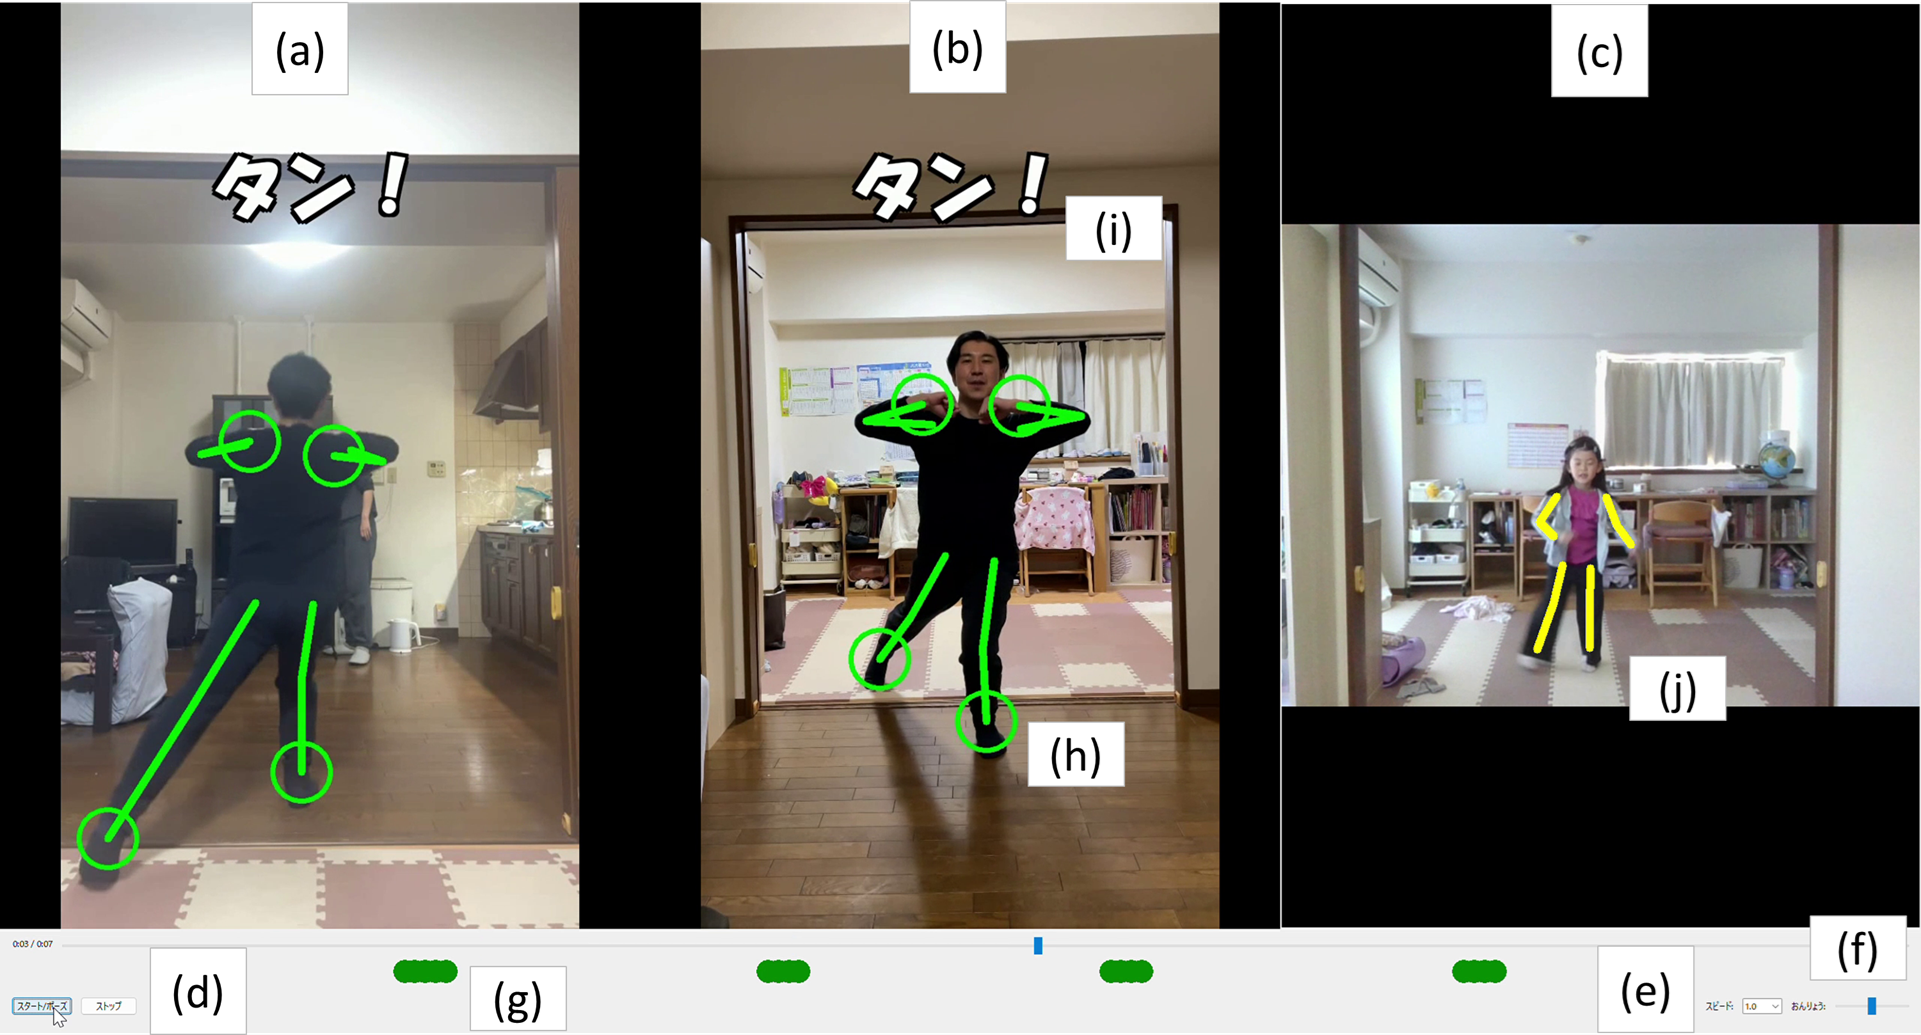
\includegraphics[width=\linewidth]{./images/UI_system_ui2.png}
  \caption{UIシステム動作画面}
  \label{fig:ui_system}
  \begin{flushleft}
    \footnotesize (a)背面動画, (b)前面動画, (c)カメラ表示, (d)動画の再生・停止, (e)動画再生速度変更, (f)音量調整, (g)「止め」タイミング印, (h)「止め」の際の骨格・図形表示, (i)オノマトペ表示, (j)カメラ動画像へのリアルタイム骨格表示
  \end{flushleft}
\end{figure}
\section{実験・評価}
\subsection{コアエンジンの実験・評価}
コアエンジンで適切に「止め」を検出できるかを確認することを目的に, 以下の実験・評価を行った. 
\subsubsection{コアエンジンの実験}
\begin{enumerate}[label=\arabic*., nosep]
  \item 評価用の動画を用意する. 本実験では5つの動画を評価用に用いた. 
  \item ダンス経験者監修のもと「止め」のフレームにアノテーションを行った. 具体的には各動画フレームを一枚ずつ画像に分割し, 「止め」のフレームだと考える動画フレームインデックスのリストを作成した.
  \item コアエンジンで「止め」のフレームを推定した. 
  \item 推定した「止め」のフレームとアノテーションした「止め」のフレームが合致するかダイスインデックス(Sørensen-Dice coefficient)によって評価した.
\end{enumerate}
 ここで, 推定した「止め」のフレームを$A$, アノテーションした「止め」のフレームを$B$とするとき, ダイスインデックスの式は以下である. 
\begin{equation}
  D(A,B)=\frac{2|A∩B|}{|A|+|B|}
\end{equation}
\begin{table*}[t]
  \centering
  \caption{コアエンジン評価 音響情報による「止め」の検出手法比較}
  \begin{tabularx}{\textwidth}{l *{10}{X}} % X列で自動幅調整
    \toprule
              & Sample1   &       & Sample2   &       & Sample3   &       & Sample4   &       & Sample5   &       \\
    \midrule
    method    & threshold &       & threshold &       & threshold &       &
    threshold &       & threshold &       \\
    \midrule
    audio     & -         & corr  & -         & corr  & -         & corr  & -         & corr  & -         & corr  \\
    \midrule
    win\_num  & win1      & win1  & win1      & win1  & win1      & win1  & win1      & win1  & win1      & win1  \\
    \midrule
    GT        & 12        & 12    & 21        & 21    & 18        & 18    & 26        & 26    & 21        & 21    \\
    cnt       & 34        & 23    & 32        & 20    & 26        & 23    & 43        & 28    & 28        & 19    \\
    TP        & 9         & 7     & 8         & 2     & 10        & 6     & 6         & 4     & 14        & 8     \\
    FP        & 25        & 16    & 24        & 18    & 16        & 17    & 37        & 24    & 14        & 11    \\
    FN        & 3         & 5     & 13        & 19    & 8         & 12    & 20        & 22    & 7         & 13    \\
    TN        & 175       & 184   & 167       & 173   & 178       & 177   & 149       & 162   & 177       & 180   \\
    Acc       & 0.868     & 0.901 & 0.825     & 0.825 & 0.887     & 0.863 & 0.731     & 0.783 & 0.901     & 0.887 \\
    Recall    & 0.750     & 0.583 & 0.381     & 0.095 & 0.556     & 0.333 & 0.231     & 0.154 & 0.667     & 0.381 \\
    Precision & 0.265     & 0.304 & 0.250     & 0.100 & 0.385     & 0.261 & 0.140     & 0.143 & 0.500     & 0.421 \\
    Dice      & 0.391     & 0.400 & 0.302     & 0.098 & 0.455     & 0.293 & 0.174     & 0.148 & 0.571     & 0.400 \\
    \bottomrule
  \end{tabularx}
\end{table*}
\subsubsection{コアエンジンの評価}
上記ダイスインデックスを用いた音響情報による「止め」の検出手法の比較と, 動画像情報による「止め」の検出手法の比較評価をそれぞれ行った. また, 動画像情報による「止め」の検出手法の評価では, 閾値アルゴリズムの閾値評価, 共通フレームの前後にフレームを拡張してダイスインデックスの値に変化があるか評価を行った. さらに, ダイスインデックスが高い事例と低い事例に関する考察も行った. \\
\textit{<表の文言整理>}\\
 ここで, 表の文言は以下の通りである. 
\begin{itemize}[nosep]
  \item method : 使用した手法. thresholdが提案手法での評価結果.
  \item win\_num : 共通フレームの前後に拡張したフレームの数. 
  \item GT : Ground truth. アノテーションしたフレームの数. 
  \item cnt : 検出したフレーム数. 
  \item TP : True Positive. 検出したフレームとGTが合致した数. 
  \item FP : False Positive. 検出したフレームとGTが合致しなかった数. 
  \item FN : False Negative. 検出しなかったフレームがGTであった数
  \item TN : True Negative. 検出しなかったフレームがGTでなかった数. 
  \item Acc : Accuracy. 精度の式は以下である. 
  \begin{equation}
    \text{Accuracy}=\frac{TP + TN}{TP+TN+FP+FN}
  \end{equation}
  \item Recall : 再現率の式は以下である.
  \begin{equation}
    \text{Recall}=\frac{TP}{TP+FN}
  \end{equation}
  \item Precision : 適合率の式は以下である.
  \begin{equation}
    \text{Precision}=\frac{TP}{TP+FP}
  \end{equation}
  \item Dice : ダイスインデックス.
\end{itemize}
\textit{<音響情報による「止め」の検出手法の評価結果>}\\
 表1に示された結果から, 振幅特徴ベース手法はダイスインデックスにおいて, 動画5つの内4つで自己相関関数ベース手法よりも高い値を示した. 特に動画2については提案手法0.302, 自己相関関数を用いた手法が0.098と大きな差が確認できる. しかし, 動画1では自己相関関数を用いた手法の方がダイスインデックスの値が高く, 動画4においては0.26ポイントしか差がない. 相対的にコアエンジンの評価実験において, 振幅特徴ベース手法の方が高いダイスインデックスを示すことから, UIシステムの実験では振幅特徴ベース手法を用いることとした. ただ, これはあくまでも今回の設定での評価であり, 動画サンプルの数を多くした場合や, 動画サンプル内の環境音やノイズが多い場合を考慮すると, よりロバストな環境でどちらを選ぶべきなのかは今後の課題である. \\
 また, 動画像情報による「止め」の検出手法の評価にて後述するが, 拡張フレーム数をwin1に, 検出アルゴリズムは閾値アルゴリズムにて評価を行った. \\
\textit{<動画像情報による「止め」の検出手法(閾値アルゴリズム)の閾値結果>}\\
 予備実験として, 閾値アルゴリズムの閾値をいくつか試し, 閾値を決定した. 表 5 2~表 5 6に示した通り, ダイスインデックスの値が最も高い10を閾値とした. この時, 拡張フレーム数はwin1とした. \\
\textit{<動画像情報による「止め」の検出手法の評価結果>}\\
 表 5 7~表 5 11に示された結果から, 閾値アルゴリズムは拡張フレーム数win1~win3のいずれにおいてもダイスインデックスが$0.174~0.571$となっており, peak検出アルゴリズムの$0.041~0.409$, k-meansアルゴリズムの$0.105~0.484$に比べて相対的に高い値を示している. 特にダイスインデックスが最も高い値を示す手法は動画1~5において全て閾値アルゴリズムとなっている. また, Accuracy, Recall, Precisionについても他の手法と比べ閾値アルゴリズムは相対的に高い値を示している. ただ, Precisionについては動画1~5において閾値アルゴリズムでも$0.140~0.500$となっており誤検出の割合が高いことが課題として挙げられる. \\
 提案手法での拡張フレーム数を変化させて行った実験では, 動画1~5に対してwin1が最もダイスインデックスが高い場合が多かった. そのため, UIシステムの実験ではwin1の設定にて実験を行う. \\
\textit{<コアエンジン評価の総括>}\\
 音響情報及び動画像情報による検出では, 各動画でダイスインデックスの値が$0.174~0.571$となり, またGTとTPから「止め」のアノテーションの約1/2を検出できたことが示され, コアエンジンの課題に寄与できたと考える. しかし, 以下考察の通り, 「止め」を検出しにくい動画への対応が今後の課題である.\\
\textit{<ダイスインデックスが高い事例と低い事例に関する考察>}\\
 今回の実験では, 動画4がどの手法も総じてダイスインデックスの値が低く, 動画5のダイスインデックスの値が最も高かった. 動画4のダンスは「止め」の動画の繰り返しでありつつも, やや流れるような動きであったため, 「止め」を検出しにくかったと考えられる. また, 動画4のダンスは身体を大きく使う振付になっており, 反動をつけるために次の動作への予備動作が比較的大きくなったと考えられる. 対して, 動画5では1拍1拍を「止め」, 身体を使う範囲が比較的狭く予備動作も少ないことから, 検出がしやすかったと考えられる. 同様の考察は \cite{ref16}でもなされており, 拍の動きにアクセントが来る振りの場合は \cite{ref16}の論文で議論されている動画分割が行いやすく, 反対に柔らかく流れるような振付に対しては分割が難しかったと述べられている. 
\subsection{UIシステムの実験・評価}
UIシステムを用いて児童・幼児にダンス練習を実施してもらい, 音声・視覚情報の有無でダンスの動きとリズムの習得度に変化があるか評価した. また, 音声・視覚情報の付与がダンス習得に有効に働いた群はどのような背景属性を持つか分析を行った. さらにアンケートにおいて音声・視覚情報の付与が児童・幼児にとって役に立ったか主観的な評価を行った. ダンス指導者へのアンケート結果についてもまとめを行った. 最後に, UIシステムの実験で収集した児童・幼児の動画から定量的にダンス習得度を評価できるか実験を行った. 
\subsubsection{UIシステムの実験}
実験参加者の属性は以下の通りである. 実験参加者の人数は16人であった. 
\begin{itemize}[nosep]
  \item 男女人数:男4人, 女12人
  \item 年齢別任数:6歳9人, 8歳6人, 9歳1人, 平均6.917歳, 標準偏差1.165 
  \item ダンス歴有無:ダンス歴有6人, ダンス歴無10人, 平均0.396年, 標準偏差0.887
\end{itemize}
 以下の通り実験参加者をグループに分け実験準備を行った(表2).
\begin{enumerate}[label=\arabic*., nosep]
  \item 実験参加者を4グループ(A, B, C, D)に分ける. 
  \item ダンスの振付を2つ(ダンスa(図 5 1), ダンスb(図 5 2))用意する. 
  \item 1つのダンスの振付について, 音声・視覚情報を付与した動画(付与有)で練習するグループと音声・視覚情報を付与しない動画(付与無)で練習するグループに分ける. 
\end{enumerate}

\begin{table}[t]
  \centering
  \caption{グループ別ダンス振付及び音声・視覚情報付与有無比較表}
  \begin{tabularx}{\linewidth}{l p{0.4\linewidth} p{0.4\linewidth}}
    \toprule
      グループ & 1回目 & 2回目 \\
    \midrule
      A & ダンスa:音声・視覚 有 & ダンスb:音声・視覚 無 \\
      B & ダンスa:音声・視覚 無 & ダンスb:音声・視覚 有 \\
      C & ダンスb:音声・視覚 有 & ダンスa:音声・視覚 無 \\
      D & ダンスb:音声・視覚 無 & ダンスa:音声・視覚 有 \\
    \bottomrule
  \end{tabularx}
\end{table}
以下の通り実験を行った. 実験参加者一人ずつ表2のグループ分けの通りの順番で練習を行った.
\begin{enumerate}[label=\arabic*., nosep]
  \item 練習するダンスを動画で2回確認する.  
  \item UIシステムでの練習前にダンス振付を行い, それを撮影する.
  \item UIシステムを使用して5分間ダンス練習を行う. 
  \item UIシステムでの練習後にダンス振付を行い, それを撮影する.
\end{enumerate}
上記を1回目, 2回目のダンスで行い, その後児童・幼児にはアンケートに回答してもらった. アンケートの項目については付録Aに示す. \\
 また, 練習前後で撮影したダンスを指導者に確認し, ダンスの動きとリズムについて評価を行った. 指導者はダンス歴22年, 指導歴16年のX氏とダンス歴13年指導歴6か月のY氏に依頼した. また指導者の方にはシステムに関するアンケートを行った(付録B).\\
\textit{<Wilcoxonの符号付順位和検定>}\\
 アンケート結果を集計し, 音声・視覚情報の有無により, 以下4つの項目について検定を行った. X氏Y氏の評価については平均値を用いた. 
\begin{enumerate}[label=\arabic*., nosep]
  \item X氏Y氏が練習前後で評価した「動きがよくできたと思いますか?」の値の差の平均値
  \item 児童・幼児が評価した「動きがよくできたと思いますか?」の値
  \item X氏Y氏が練習前後で評価した「リズムはよくできたと思いますか?」の値の差の平均値
  \item 児童・幼児が評価した「リズムはよくできたと思いますか?」の値
\end{enumerate}
上記については, 次の略称を以後使用する. 「1. X氏Y氏A(平均)」, 「2. 児童・幼児 A」, 「3. X氏Y氏R(平均)」, 「4. 児童・幼児 R」. 
 音声・視覚情報の有無による2群間で母集団の中央値に差があるかを検定するため, ノンパラメトリック手法であるWilcoxonの符号付順位和検定(Wilcoxon signed-rank test)を実施した. 本検定はデータが正規分布に従わない場合でも有効であり, 本実験のような状況にも適している. 具体的な手順としては, 各ペアの差$d_{i}=x_{i}-y_{i} (i=1,\dots,N)$を計算し, 差が0でないものを抽出した. その際, 差が0のデータについては有効サンプル数($N$)から除外した. その後, 絶対値$|d_{i}|$に対して昇順に順位(rank)を付け, 元の符号(正負)を順位に戻した. 正の符号に対応する順位の総和$W^+$および負の符号に対応する順位の総和$W^-$を算出した. 検定統計量$W$は, これらのうちの小さい方$(W=min⁡(W^+,W^-))$を採用し, これを用いて「中央値に差がない」とする帰無仮説の検定を行った. 検定は両側検定で有意水準$p=0.05 or 0.01$にて行った. 統計量$W$が$N$数に応じて,表 5 13の数値のとき, 統計的有意差があると判断する. この統計表はScipy \cite{ref27}のscipy.stats.wilcoxonを用いて作成した. \\
\textit{<音声・視覚情報の付与が有効に働いた群の背景分析>}\\
 また, 今回実験したデータに対して解析を行った. 解析は, 被験者の背景属性および児童・幼児の自己評価項目について, 音声・視覚情報の付与が有効であった群(Snd\_Vis-oriented), 音声・視覚情報の付与のない方が有効であった群(Non-Snd\_Vis-oriented), および両者に差が見られなかった群(Balanced)の3カテゴリに分類し, それぞれの特徴を5段階スケールのレーダーチャートにより可視化した. まず, 音声・視覚情報の付与によるダンス習得効果を示す4つの評価指標(音声・視覚情報有無それぞれの「音声・視覚情報有X氏Y氏A(平均)」, 「音声・視覚情報有X氏Y氏R(平均)」, 「音声・視覚情報無X氏Y氏A(平均)」, 「音声・視覚情報無X氏Y氏R(平均)」の4項目)に基づき, 各被験者に音声・視覚情報有りの総合得点$SV_{i}$と音声・視覚情報無しの総合得点$NSV_{i}$を以下の式により算出した$(i=1,\dots,16)$:
\begin{equation}
  SV_{i}=\sum_{j}^{4}sv_{ij},\; NSV_{i}=\sum_{j}^{4}nsv_{ij}
\end{equation}
ここで, $sv_{ij}$および$nsv_{ij}$は, それぞれ音声・視覚情報有無の各指標である. 次に, 音声・視覚情報有無の得点差$D_{i}=SV_{i}-NSV_{i}$に基づき, 以下の基準カテゴリを付与した:
\begin{itemize}[nosep]
  \item $D_{i} \geq 0.5$ : Snd\_Vis-oriented群
  \item $D_{i} \leq 0.5$ : Non-Snd\_Vis-oriented群
  \item 上記以外 : Balanced群
\end{itemize}
このカテゴリ分類に基づき, 以下の7項目を対象に平均値を算出した:
\begin{itemize}[nosep]
  \item 背景属性:性別(gender), 年齢(age), ダンス歴(dance history)
  \item 児童・幼児自己評価項目:\\
        音声・視覚情報有\_動き(snd\_vis\_Act\_child),\\
        音声・視覚情報有\_リズム(snd\_vis\_Rhy\_child),\\
        音声・視覚情報無\_動き(Non-snd\_vis\_Act\_child),\\
        音声・視覚情報無\_リズム(Non-snd\_vis\_Rhy\_child) 
\end{itemize}
上記のうち, 性別・年齢・ダンス歴の3項目は尺度が異なるため, 5段階にスケーリングした. これにより, すべての指標を5段階スケールで視覚的に比較可能な形式に統一した. 最終的にカテゴリごとの平均ベクトルをレーダーチャート上にプロットし, 各群の傾向を視覚化した. \\
\textit{<アンケートによる音声・視覚情報付与手法別の主観的評価分析>}\\
 さらに, アンケートにおいて音声・視覚情報の付与が児童・幼児にとって役に立ったか主観的な評価を行い, 表にまとめた. \\
\textit{<ダンス指導者へのアンケートまとめ>}\\
 ダンス指導者へ実施したアンケートを表にまとめた. \\
\textit{<児童・幼児の動画分析による定量的評価実験>}\\
 最後に, UIシステム実験で収集した練習前後の児童・幼児のダンス動画をコアエンジンで分析し, 定量的にダンス習得度が評価できるか実験を行った. 
\subsubsection{UIシステムの評価}
\begin{table}[t]
  \centering
  \caption{音声・視覚情報の有無によるWilcoxonの符号付順位和検定結果}
  \begin{tabularx}{\linewidth}{X c c c c}
    \toprule
      項目 & N & W & p=0.05 & p=0.01 \\
    \midrule
      1. X氏Y氏A(平均) & 12 & 37.5 & - & - \\
      2. 児童・幼児 A & 14 & 36.5 & - & - \\
      3. X氏Y氏R(平均) & 12 & 28 & - & - \\
      4. 児童・幼児 R & 9 & 20 & - & - \\
    \bottomrule
  \end{tabularx}
\end{table}
\textit{<Wilcoxonの符号付順位和検定>}\\
 音声・視覚情報の有無によるWilcoxonの符号付順位和検定結果は表 5 14の通りである. 4項目すべてにおいて有意差はみられなかった. すなわち, いずれの評価においても, 音声・視覚情報の付与による学習効果の違いは統計的に有意な変化を示さなかった. この結果は, 音声・視覚情報の有無が主観的な動作評価やリズム評価に与える影響が限定的である可能性を示唆している. 特に, 児童・幼児自身の評価(項目2および4)においても顕著な差が認められなかったことから, 音声・視覚情報の付与が学習者自身の動作感覚の変化に直結しない可能性がある. また, X氏およびY氏による評価においても一貫して非有意であったことは, 観察者による外的評価においても同様の傾向が見られることを意味する. \\
 これらの結果は, 今回の実験設定(回数)では音声・視覚情報の提示が必ずしも学習成果の向上につながるとは限らないこと, あるいは提示方法やタイミングなど, 他の要因が効果に影響している可能性を示唆する. \\
\begin{figure}[t]
  \centering
  % ページ幅の50%に縮小
  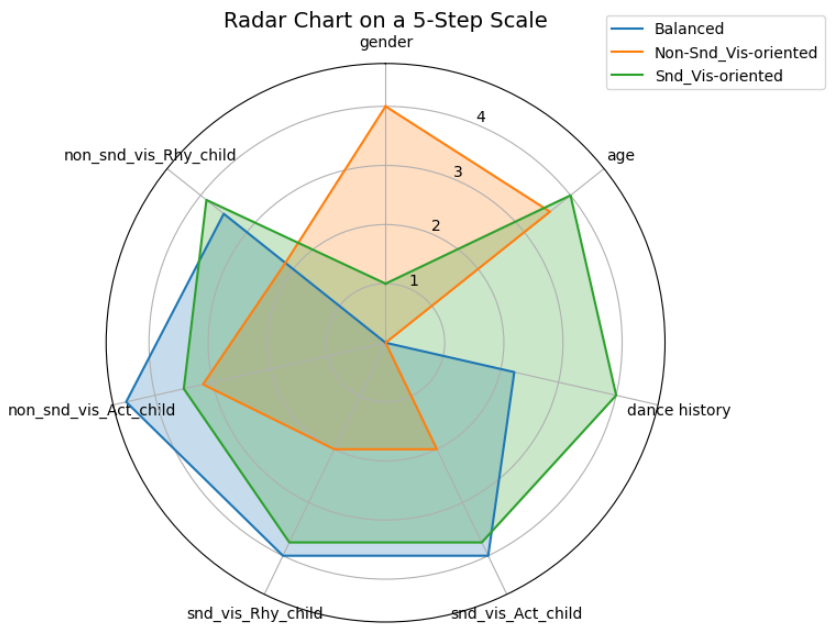
\includegraphics[width=0.45\textwidth]{./images/radar_chart.png}
  \caption{音声・視覚情報有無による有効群ごとの背景情報レーダーチャート}
  \label{fig:radar_chart}
\end{figure}
\textit{<音声・視覚情報の付与が有効に働いた群の背景分析>}\\
 次に, 音声・視覚情報の付与が有効であった群(Snd\_Vis-oriented, $n=8$), 音声・視覚情報の付与のない方が有効であった群(Non-Snd\_Vis-oriented, $n=6$), および両者に差が見られなかった群(Balanced, $n=2$)の3群について, 各群の性別・年齢・ダンス歴と自己評価項目との関連性を分析した(図3,表4). ここで,表4は図3の数値を表にまとめたものである. また, 表の性別・年齢・ダンス歴は正規化前の実際の平均値を使用している.\\
\begin{table*}[t]
  \centering
  \caption{音声・視覚情報有無による有効群ごとの背景情報表}
  \begin{tabularx}{\textwidth}{>{\raggedright}X *{8}{X}} % 1列目だけ左揃え
    \toprule
      & 人数 & 1女, 2男 & 年齢 & ダンス歴(年) 
      & \multicolumn{2}{c}{snd\_vis} 
      & \multicolumn{2}{c}{Non-snd\_vis} \\
      \cmidrule(lr){6-7} \cmidrule(lr){8-9}
      &     &     &     &     
      & Act\_child & Rhy\_child & Act\_child & Rhy\_child \\
    \midrule
      \hbox{Snd\_Vis oriented} & 8 & 1.13 & 7.13 & 1.34 & 3.75 & 3.75 & 3.50 & 3.88 \\
      \hbox{Non-Snd\_Vis oriented} & 6 & 1.50 & 7.00 & 0.00 & 2.00 & 2.00 & 3.17 & 2.17 \\
      \hbox{Balanced} & 2 & 1.00 & 6.00 & 0.75 & 4.00 & 4.00 & 4.50 & 3.50 \\
    \bottomrule
  \end{tabularx}
\end{table*}
\textbf{\rule{1ex}{1ex}\; Snd\_Vis-oriented群の特徴}\\
 Snd\_Vis-oriented群($n=8$)は, 性別平均が1.13(≒女子中心), 年齢7.13歳, ダンス歴1.34年と, 他群と比較してダンス経験が長く, 年齢も高めであった. また, 自己評価においても「snd\_vis\_Act\_child」と「snd\_vis\_Rhy\_child」の得点がいずれも3.75と高く, 音声・視覚情報提示に対する感受性が高い傾向が見られた. 加えて, 自己評価スコア「non\_snd\_vis\_Act\_child」(3.50), 「non\_snd\_vis\_Rhy\_child」(3.88)も一定以上であり, 全体的に自己評価の高い児童・幼児で構成されていると解釈できる.\\
\textbf{\rule{1ex}{1ex}\; Non-Snd\_Vis-oriented群の特徴}\\
 Non-Snd\_Vis-oriented群($n=6$)は, 性別平均が1.50(≒男子中心), 年齢7.00歳, ダンス歴0.00年であり, 未経験の男子児童が主に該当した. 自己評価において, 「non-snd\_vis\_Act\_child」は3.17と一定の高さを示した一方, 「snd\_vis\_Act\_child」と「snd\_vis\_Rhy\_child」はともに2.00と低く, 音声・視覚情報提示による効果が出にくい層といえる.\\
\textbf{\rule{1ex}{1ex}\; Balanced群の特徴}\\
 Balanced群($n=2$)は, 性別平均1.00(女子のみ), 年齢6.00歳, ダンス歴0.75年と, 年齢・経験ともに中間的な位置にある. 自己評価スコアはいずれも高く, 「snd\_vis\_Act\_child」と「snd\_vis\_Rhy\_child」は4.00, また, 「non\_snd\_vis\_Act\_child」は4.50, 「non\_snd\_vis\_Rhy\_child」は3.50と高水準にあった. これは, 音声・視覚情報付与いかんによらず, 柔軟に適応できる学習者像を示していると考えられる. \\
 これらの結果は, 児童・幼児において, 性別やダンス経験年数によって音声・視覚情報の有無が学習効果に与える影響が異なる可能性を示唆している. 特に以下のようなことが考えられる. 
\begin{itemize}[nosep]
  \item ダンス経験のある女子児童には動画への音声・視覚情報の付与が有効
  \item 未経験かつ男子児童には, 音声・視覚情報の付与の効果は限定的
  \item 音声・視覚情報の付与いかんに関わらず高得点を示す児童には状況に応じたダンス習得が望ましい. 
\end{itemize}
 また, 児童・幼児に「システムをもっとよくするためにこうした方がいいと思うところはありますか?」とアンケートしたところ, Non-Snd\_Vis-oriented群の児童・幼児から, 「カメラ表示の記号の〇と棒が混乱してしまった.」, 「ダンスのことがわからない.」という意見があった. さらに, Balanced群の児童・幼児からは「先生の動きにもっとあわせられるシステムだとよかった.」との意見があった. 考察として, ダンス未経験の児童・幼児はどこに意識を集中するかのイメージが難しく, 本提案システムはある程度ダンス経験がある方が有効である可能性がある.\\
\textit{<アンケートによる音声・視覚情報付与手法別の主観的評価分析>}\\
 さらに, 音声・視覚情報の付与が児童・幼児にとって役立ったかの主観的な評価について表5にまとめる. \\
\begin{table}[t]
  \centering
  \caption{児童・幼児による音声・視覚情報付与手法の主観的評価}
  \begin{tabularx}{\linewidth}{X c c c c c}
    \toprule
      & Ave & StDev & Max & Min & Median \\
      見本動画 & 3.938 & 0.937 & 5 & 3 & 4 \\
      カメラ表示 & 4.063 & 1.128 & 5 & 2 & 4.5 \\
      オノマトペの音 & 3.625 & 1.557 & 5 & 1 & 4 \\
      システム & 4.125 & 0.953 & 5 & 3 & 4.5 \\
    \bottomrule
  \end{tabularx}
\end{table}
 ここで, 表の文言は付録Aの以下質問項目の略称である. 
\begin{itemize}[nosep]
  \item 見本動画 : 見本動画の文字や記号はダンス練習の役に立ちましたか?
  \item カメラ表示 : カメラ表示の記号はダンス練習の役に立ちましたか?
  \item オノマトペの音 : オノマトペの音(タン)はダンス練習の役に立ちましたか?
  \item システム : またシステムを使いたいと思いますか?
\end{itemize}
また, それぞれについて平均値(Ave), 標準偏差(StDev), 最大値(Max), 最小値(Min), 中央値(Median)を算出した. \\
 平均値に着目すると, 「システム」が最も高く(4.125), 次いで「カメラ表示」(4.063), 「見本動画」(3.938), 「オノマトペの音」(3.625)の順となっており, 視覚的補助(カメラ表示, 見本動画)に対する評価が音声的補助(オノマトペ)よりも高い傾向が見られた. 一方で, 評価のばらつきを示す標準偏差に着目すると, 「オノマトペの音」が最も大きく(1.557), 児童・幼児間での評価の個人差が顕著であることが示唆される. 最小値も1.000と, 他の項目に比べて顕著に低い. このことから, オノマトペによる提示は一部の児童・幼児にとっては理解や需要が難しい可能性がある. 一方で「見本動画」の標準偏差は1.0未満であり, 「カメラ表示」も「オノマトペの音」よりも標準偏差が低いことから, 視覚的補助は比較的安定した評価が得られている. また, 「システム」は標準偏差が0.953であり, 児童・幼児には満足度が高い結果となったため, 練習の習慣化にも使用できる可能性が示唆された. \\
 以上の結果から, 視覚的な情報提示(「見本動画」, 「カメラ表示」)は児童・幼児に対して有効であり, かつ評価のばらつきが小さいことから一貫した学習支援手法として有望であると考えられる. 一方で, オノマトペの音声提示については, 平均値が4.0に近い水準を示しながらもばらつきが大きく, 個別の特性や学習スタイルに応じた柔軟な運用が求められる手法であるといえる. \\
\textit{<ダンス指導者へのアンケートまとめ>}\\
 ダンス指導者へ実施したアンケート(付録B )を表 5 17にまとめた. システムの改善点として「ステップ練習において, 足の動きの順序が視覚的に分かる情報からの映像があると望ましい」との意見が寄せられた. 本システムでは前面及び背面からの見本動画のみを使用していたが, 足の動きがダンス習得において重要な構成要素であることを踏まえると, 上方からの映像を取り入れた教材の開発も今後の重要な課題である.\\
\textit{<児童・幼児の動画分析による定量的評価実験>}\\
 最後に, UIシステム実験で収集した練習前後の児童・幼児のダンス動画をコアエンジンで分析した結果を表 5 18~表 5 20にまとめた. 「a\_pre」, 「a\_pst」, 「b\_pre」,「 b\_pst」はそれぞれ「ダンスaの練習前」, 「ダンスaの練習後」, 「ダンスbの練習前」, 「ダンスbの練習後」を表している. 評価については, Snd\_Vis-oriented群, Non-Snd\_Vis-oriented, Balanced群から各1名ずつ抽出しコアエンジンの処理にかけ, 抽出した動画フレームとGTである見本動画の抽出フレームにてダイスインデックスを比較した. 結果としては定量的な評価を行うにはいくつかの課題があることが判明した. \\
 一つは, 見本動画との動作の同期に関する問題である. 児童・幼児がある程度見本と同じリズムで動作できた場合には, メトロノーム音および初回の「止め」の動作を基準に同期をはかり, 評価を行うことが可能であった. しかし, 特に初心者においてはリズムに乗ること自体が困難であり, 評価の基準点を特定できないケースが散見された. (今回の動画では, 初回の「止め」の動画フレームにて同期させた) また, 「止め」の姿勢を検出する設計により, 実際には動作が伴っていない場合でも「止め」として誤検出され, 評価が成立しない問題も確認された. 具体的には, 完全に止まっている動画のダイスインデックスが高く, 評価が良いと判断されたしまっていた. これに対して, 見本と類似した座標に手足が位置していることを条件とした「止め」の評価基準の導入など, 今後の改善が求められる.
\section{おわりに}
\subsection{まとめ}
本研究では, ヒップホップダンスにおける「止め」の動きに着目し, 動画上の「止め」の瞬間に音声・視覚情報を付与することで, 児童・幼児のダンス習得を支援するシステムを提案した. 提案手法は大きくコアエンジンとUIシステムとに大別され, コアエンジンでは動画を入力として音響情報と動画像情報により「止め」の動作を行っている動画フレームを検出し, UIシステムでは検出した動画フレームに音声・視覚情報を付与することができた. UIシステムを使用した児童・幼児に対する比較実験では, 音声・視覚情報を付与してダンス練習を行った群と音声・視覚情報を付与しないでダンス練習を行った群で統計的有意差が認められるか検定を行った. 音声・視覚情報の有無で統計的な有意差はみられなかったが, 音声・視覚情報の付与を行うことがダンス習得に有効な児童・幼児の背景属性を分析することができた. また, 児童・幼児のシステムへの満足度が高く, 練習に不可欠な継続性の可能性を見いだせたこと, 視覚情報の付与が学習支援として有効であること, 音声情報の付与は児童・幼児の特性を考慮して選択的に使用する必要性があることなどの示唆が得られた. \\
 本研究の主な貢献は以下の3点である.
\begin{itemize}[nosep]
  \item ダンス動画から「止め」の姿勢を自動的に検出する手法の提案. 
  \item 児童・幼児を対象とした, 「止め」の姿勢とタイミングの理解を促すダンス習得支援システムの構築. 
  \item 音声および視覚情報の有無によるダンス習得度の違いに関する実証的評価.
\end{itemize}
\subsection{今後の課題}
本提案手法におけるコアエンジン及びUIシステムには以下のような課題が残されている. \\
 まず, コアエンジンおよびUIシステムの共通の課題として, 評価用サンプル数が少ない点が挙げられる. このため, コアエンジンにおいては, 今回のUIシステムで使用した手法以外に, よりロバストに動作を検出できる可能性がある. 音響情報による2手法および動画像情報による3手法について, サンプル数の増加による精度検証が必要である. 一方, UIシステムでは被験者が16名と少なく, 統計的検定結果の信頼性に影響を及ぼした可能性がある. したがって, 今度はより多くのサンプルを収集し, 再検証を行う必要がある. \\
 次に, 本研究では撮影された児童・幼児のダンス動画に対して, コアエンジンを用いた定量的評価を行う際に, いくつかの技術的課題があった. 一つは, 見本動画との動作の同期に関する問題, 二つ目は, 実際には動作が伴っていない場合でも「止め」として誤検出され, 評価が成立しない問題である. 今後の改善点として, 見本に類似した動画像上の座標に手足が位置していることを条件とする「止め」の評価基準の導入が求められる.\\
 さらに, ダンス指導者へのアンケートから, システムの改善点の意見が寄せられた. 本システムで取り入れきれなかった部分の開発も今後の重要な課題である. 

\ack %% 謝辞
実験データの提供および評価にご協力いただいたDANCE STUDIO NESTの先生方, ならびに実験データ収集にご協力くださった児童・幼児とその保護者の皆様にも, この場を借りて深く御礼申し上げます. 

\bibliographystyle{sieicej}
\bibliography{myrefs}
% \begin{thebibliography}{99}% 文献数が10未満の時 {9}
% \bibitem{}
% \end{thebibliography}

% \appendix
% \section{}

%% 著者紹介・顔写真の掲載はC分冊の場合は任意です.
% \begin{biography}
% \profile*{}{}{}U
%\profile{会員種別}{名前}{紹介文}% 顔写真あり
%\profile*{会員種別}{名前}{紹介文}% 顔写真なし
% \end{biography}

\end{document}
